% move all configuration stuff into one file so we can focus on the content
\documentclass[aspectratio=169,hyperref={pdfpagelabels=false,colorlinks=true,linkcolor=white,urlcolor=blue},t]{beamer}

%%%%%%%%%%%%%%%%%%%%%%%%%%%%%%%%%%%%%%%%%%%%%%%%%%%%%%%%%%%%%%%%%%%%%%%%%%%%%%%%%%
%%%%%%%%%%%%%%%%%%%%%%%%%%%%%%%%%%%%%%%%%%%%%%%%%%%%%%%%%%%%%%%%%%%%%%%%%%%%%%%%%%
% packages
\usepackage{pict2e}
\usepackage{epic}
\usepackage{amsmath,amsfonts,amssymb}
\usepackage{units}
\usepackage{fancybox}
\usepackage[absolute,overlay]{textpos} 
\usepackage{media9} % avi2flv: "C:\Program Files\ffmpeg\bin\ffmpeg.exe" -i TuneFreqFilterbank.avi -b 600k -s 441x324 -r 15 -acodec copy TuneFreqFilterbank.flv
\usepackage{animate}
\usepackage{gensymb}
\usepackage{multirow}
\usepackage{silence}
\usepackage[backend=bibtex,style=ieee]{biblatex}
\AtEveryCitekey{\iffootnote{\tiny}{}}
\addbibresource{references}

%%%%%%%%%%%%%%%%%%%%%%%%%%%%%%%%%%%%%%%%%%%%%%%%%%%%%%%%%%%%%%%%%%%%%%%%%%%%%%%%%%
%%%%%%%%%%%%%%%%%%%%%%%%%%%%%%%%%%%%%%%%%%%%%%%%%%%%%%%%%%%%%%%%%%%%%%%%%%%%%%%%%%
% relative paths
\graphicspath{{graph/}}


%%%%%%%%%%%%%%%%%%%%%%%%%%%%%%%%%%%%%%%%%%%%%%%%%%%%%%%%%%%%%%%%%%%%%%%%%%%%%%%%%%
%%%%%%%%%%%%%%%%%%%%%%%%%%%%%%%%%%%%%%%%%%%%%%%%%%%%%%%%%%%%%%%%%%%%%%%%%%%%%%%%%%
% units
\setlength{\unitlength}{1mm}

%%%%%%%%%%%%%%%%%%%%%%%%%%%%%%%%%%%%%%%%%%%%%%%%%%%%%%%%%%%%%%%%%%%%%%%%%%%%%%%%%%
%%%%%%%%%%%%%%%%%%%%%%%%%%%%%%%%%%%%%%%%%%%%%%%%%%%%%%%%%%%%%%%%%%%%%%%%%%%%%%%%%%
% theme & layout
\usetheme{Frankfurt}
\beamertemplatenavigationsymbolsempty
%\setbeamertemplate{frametitle}[smoothbars theme]
\setbeamertemplate{frametitle}
{
    \begin{beamercolorbox}[ht=1.8em,wd=\paperwidth]{frametitle}
        \vspace{-.1em}%
        \hspace{.2em}{\strut\insertframetitle\strut}
        
        \hspace{.2em}\small\strut\insertframesubtitle\strut
        %\hfill
        %
\includegraphics[height=.8cm,keepaspectratio]{CenterMusicTechnology-solid-2lines-white-CoAtag}
        
    \end{beamercolorbox}
    \begin{textblock*}{100mm}(11.6cm,.7cm)
        \includegraphics[height=.8cm,keepaspectratio]{logo_GTCMT_black}
    \end{textblock*}
}

% set this to ensure bulletpoints without subsections
\usepackage{remreset}
\makeatletter
\@removefromreset{subsection}{section}
\makeatother
\setcounter{subsection}{1}

%---------------------------------------------------------------------------------
% appearance
\setbeamercolor{structure}{fg=gtgold}
\setbeamercovered{transparent} %invisible
\setbeamercolor{bibliography entry author}{fg=black}
\setbeamercolor*{bibliography entry title}{fg=black}
\setbeamercolor*{bibliography entry note}{fg=black}

%\usepackage{pgfpages}
%\setbeameroption{show notes}
%\setbeameroption{show notes on second screen=right}
%---------------------------------------------------------------------------------
% fontsize
\let\Tiny=\tiny

%%%%%%%%%%%%%%%%%%%%%%%%%%%%%%%%%%%%%%%%%%%%%%%%%%%%%%%%%%%%%%%%%%%%%%%%%%%%%%%%%%
%%%%%%%%%%%%%%%%%%%%%%%%%%%%%%%%%%%%%%%%%%%%%%%%%%%%%%%%%%%%%%%%%%%%%%%%%%%%%%%%%%
% warnings
\pdfsuppresswarningpagegroup=1
\WarningFilter{biblatex}{Patching footnotes failed}
\WarningFilter{latexfont}{Font shape}
\WarningFilter{latexfont}{Some font shapes}
\WarningFilter{gensymb}{Not defining}



\subtitle{Part 7.2: Temporal Analysis}

%%%%%%%%%%%%%%%%%%%%%%%%%%%%%%%%%%%%%%%%%%%%%%%%%%%%%%%%%%%%%%%%%%%%%%%%%%%%
\begin{document}
    % generate title page
	

\begin{frame}
    \titlepage
    %\vspace{-5mm}
    \begin{flushright}
        \href{http://www.gtcmt.gatech.edu}{\includegraphics[height=.8cm,keepaspectratio]{logo_GTCMT_black}}
    \end{flushright}
\end{frame}


    \section[overview]{lecture overview}
        \begin{frame}{temporal analysis}{overview}
            \begin{itemize}
                \item   \textbf{text book}  
                    \begin{itemize}
                        \item   \href{http://ieeexplore.ieee.org/xpl/articleDetails.jsp?tp=&arnumber=6331123&}{\underline{\textit{Chapter 6: Temporal Analysis} (pp.~134--137)}}
                    \end{itemize}
                \bigskip
                \item<2->   \textbf{lecture content}
                    \begin{itemize}
                        \item<2->   time signature \& downbeat detection
                        \item<3->   features and rhythm description
                    \end{itemize}
            \end{itemize}
        \end{frame}


        \section[meter]{meter \& downbeat detection}
            \begin{frame}{meter \& downbeat detection}{brainstorm}
                \question{what are your ideas for detecting the meter, time signature, and downbeats in a complex mixture}
            \end{frame}
            \begin{frame}{meter \& downbeat detection}{introduction}
                \begin{itemize}
                    \item   relation of meter and downbeat is comparable to relation between tempo and beat phase
                    \item   meter and downbeat are on a higher hierarchical level
                    \smallskip
                    \item<2-> extraction can be very similar but on different periodicity scale
                        \begin{enumerate}
                            \item   extraction of novelty function
                            \item   estimation of bar period
                            \item   estimation of downbeat
                        \end{enumerate}
                \end{itemize}
            \end{frame}
            \begin{frame}{meter \& downbeat detection}{variants}
                \begin{enumerate}
                    \item	\textbf{novelty function}
                        \begin{itemize}
                            \item   onset probability
                            \item   downbeat-specific (may be genre-dependent)
                                \begin{itemize}
                                    \item   bass onset/energy increase
                                    \item   pitch chroma change
                                    \item   beat and onset match
                                \end{itemize}
                        \end{itemize}
                    \smallskip
                    \item<2->	\textbf{quantization to beat or tatum}
                    \smallskip
                    \item<3->	\textbf{periodicity estimation}
                        \begin{itemize}
                            \item   ACF
                            \item   spectrum
                        \end{itemize}
                    \smallskip
                    \item<4->	\textbf{downbeat estimation} 
                        \begin{itemize}
                            \item   delta pulse CCF
                            \item   \ldots
                        \end{itemize}
                \end{enumerate}
            \end{frame}

        \section[features]{low level features and representations}
            \begin{frame}{beat histogram}{introduction}
                \vspace{-3mm}
                \textbf{beat spectrum}/\textbf{beat histogram}: compact representation of periodicities
                \begin{columns}[T]
                    \column{.55\linewidth}
                        \begin{enumerate}
                            \item<2->   compute novelty function
                                \begin{itemize}
                                    \item   time domain features: envelope, rms
                                    \item   spectral differences: flux, ...
                                    \item   any other feature
                                \end{itemize}
                            \item<3->   compute transform
                                \begin{itemize}
                                    \item   (resonance) filter bank
                                    \item   magnitude spectrum
                                    \item   pick onsets\\ $\rightarrow$ compute histogram of Inter-Onset-Intervals 
                                \end{itemize}
                        \end{enumerate}
                    \column{.45\linewidth}
                        \begin{figure}
                            \centering
                                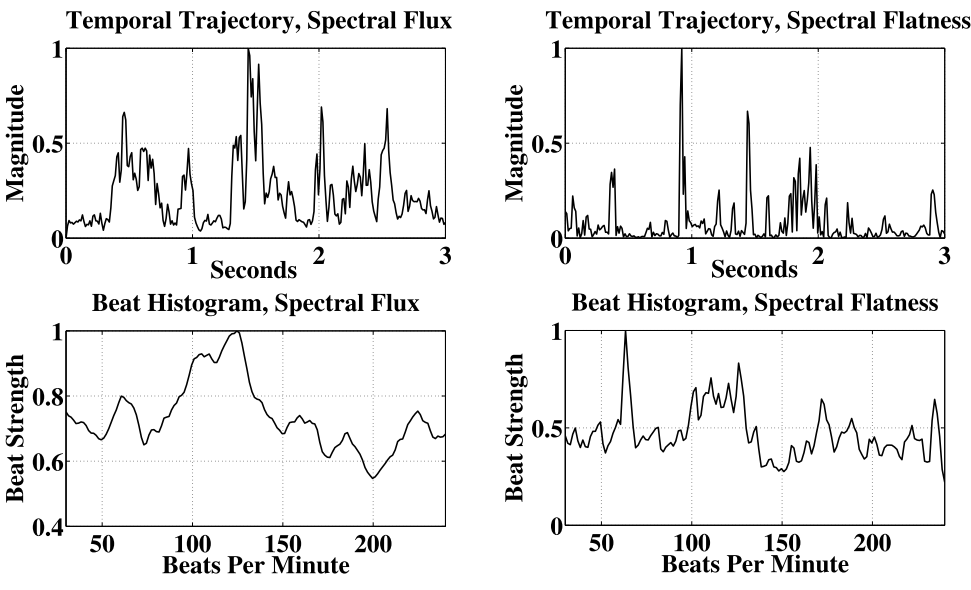
\includegraphics[scale=.2]{lykartsis_beathistogram}
                        \end{figure}
                \end{columns}
                
                \flushright{graph from \footfullcite{lykartsis_rhythm_2015}}
            \end{frame}
            \begin{frame}{beat histogram}{feature examples}
                
                \begin{itemize}
                    \item	\textbf{statistical features} 
                        \begin{itemize}
                            \item mean, centroid, standard deviation, kurtosis, \ldots
                        \end{itemize}
                    \item<2->   \textbf{peak features}
                        \begin{itemize}
                            \item   value and position of absolute max
                            \item   ratio (value and position) of strongest and 2nd strongest peaks
                        \end{itemize}
                    \item<3->	\textbf{other features}
                        \begin{itemize}
                            \item   flatness, crest, high frequency content, MFCCs (??),\ldots
                            \item   features from ACF of beat histogram\footfullcite{burred_hierarchical_2004}
                            
                            \only<3->{  \begin{center}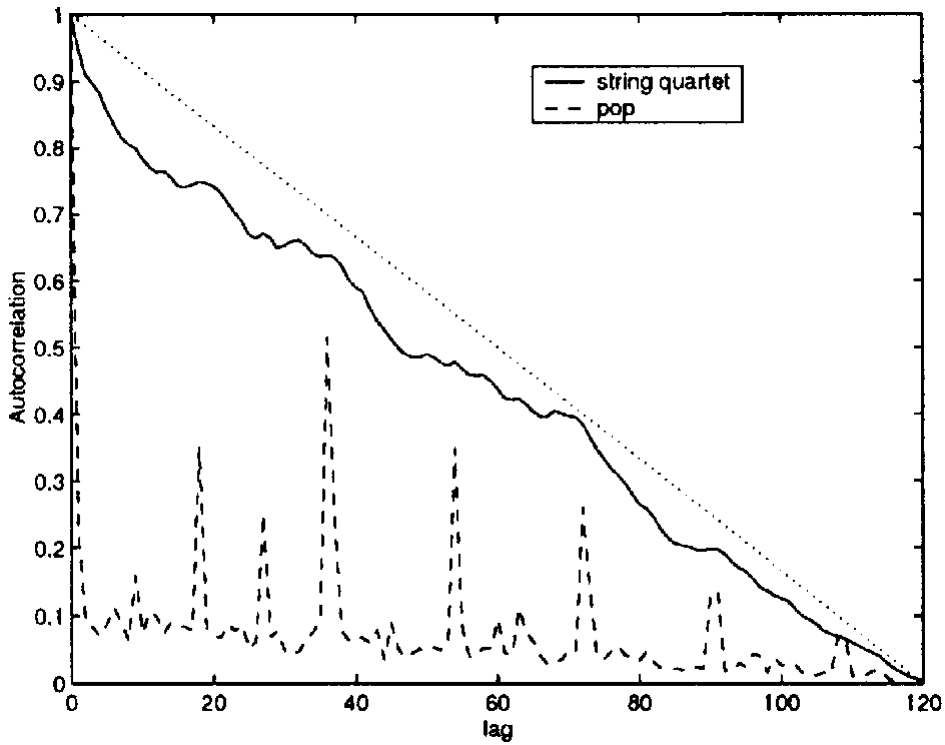
\includegraphics[scale=.15]{burred_acfofbeathisto}\end{center}}
                        \end{itemize}
                        \vfill
                        
                \end{itemize}
            \end{frame}

        \section[summary]{lecture summary}
        \begin{frame}{summary}{lecture content}
            \begin{enumerate}
                \item   how to detect the time signature with a given meter
                \smallskip
                \item<2->   name commonalities and differences between beat detection and downbeat detection
                \smallskip
                \item<3->   name examples of low level features describing temporal properties
            \end{enumerate}
        \end{frame}
\end{document}

